\subsection{E4: learned codes attain the floor}
\label{sec:res-e4}

Gradient descent under the unit-diagonal constraint drives the interface to the floor
(Table~\ref{tab:e4}, Fig.~\ref{fig:e4}). Over
\EfourFreeRuns{} runs of the free variant, spanning all \EfourConfigs{} configurations, the
attainment ratio reaches a mean of \EfourFreeRatioMean{} and never exceeds
\EfourFreeRatioMax, with \EfourFreeBelowFloor{} runs below the floor. The tied variant is
sharper still: over \EfourTiedRuns{} runs, mean ratio \EfourTiedRatioMean{} with a maximum of
\EfourTiedRatioMax{} (\EfourTiedBelowFloor{} below the floor), and a relative tight-frame
residual of \EfourTiedFrameResidualMean{} on average (worst case
\EfourTiedFrameResidualMax). In other words, the optimiser recovers the equality case of
Proposition~\ref{prop:tight}: a unit-norm tight frame emerges from gradient descent rather than
being constructed.

The smooth-max variant is the one that does \emph{not} reach its target, and the reason is
structural rather than a tuning failure. Over \EfourSoftmaxRuns{} runs it attains a mean
mean-square ratio of \EfourSoftmaxRatioMean{} (worst case \EfourSoftmaxRatioMax,
\EfourSoftmaxBelowFloor{} below the floor) and drives the maximum off-diagonal entry only to
\EfourSoftmaxRatioMaxMean{} times $\sqrt{W(F,d)}$. Equality in the maximum form requires an
equiangular tight frame, and those exist only for special $(d,F)$ --- none of our
\EfourConfigs{} configurations is guaranteed to admit one. The maximum form of the bound is
therefore approached but not attained here, which is the expected outcome and not evidence
against the bound.

The uncalibrated ablation is the most informative of the four, and its outcome is more extreme
than we expected. Removing the diagonal constraint does not lead the optimiser to a code with
low interference: it leads it to the trivial solution. Across all \EfourUncalRuns{} runs the
\emph{raw} off-diagonal energy collapses to \EfourUncalRawRatioMean{} --- the readout is driven
to zero --- and with it the diagonal gains, whose smallest absolute value reaches
\EfourUncalGainMin{} in single precision. In \EfourUncalDegenerate{} of the
\EfourUncalRuns{} runs the calibration is therefore undefined and Algorithm~\ref{alg:one}
returns \textsc{Degenerate}; in the remaining runs the calibrated interface still respects the
floor, and in no run did it fall below (\EfourUncalBelowFloor{} violations). An unconstrained
optimiser reports spectacular apparent cross-talk while destroying the interface it was
supposed to build. This is Remark~\ref{rem:calib} as an experiment, and it is the reason
step~4 of Algorithm~\ref{alg:one} exists and reports a status rather than a number.

\begin{figure}[t]
\centering
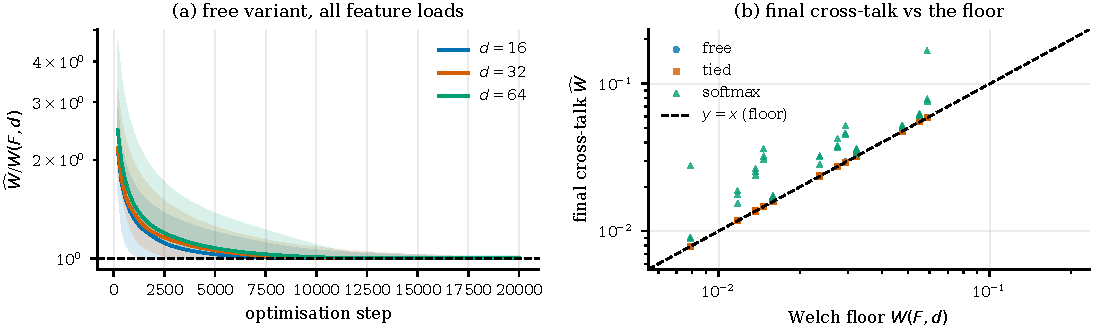
\includegraphics[width=\linewidth]{figures/fig2_optimized_codes.pdf}
\caption{\textbf{Optimised codes attain the Welch floor.} (a) Attainment ratio during
optimisation of the free variant; bands are min--max over configurations and seeds.
(b) Final cross-talk against the floor across every configuration and variant; the dashed line
is equality. Generated by \code{scripts/make\_figures.py} from \code{results/e4}.}
\label{fig:e4}
\end{figure}

\begin{table}[t]
\centering
\caption{E4: attainment of the floor by gradient-optimised codes, \EfourRuns{} runs over
\EfourConfigs{} configurations. ``Below floor'' counts runs whose calibrated interface fell
under the theoretical bound; it must be zero. The uncalibrated ablation has no meaningful
calibrated ratio by construction.}
\label{tab:e4}
\small
% Generated by scripts/make_tables.py from results/. Do not edit by hand.
\begin{tabular}{lrrrrr}
\toprule
variant & runs & mean $\widehat{W}/W$ & max $\widehat{W}/W$ & below floor & extra \\
\midrule
free ($G$, $\Phi$ independent) & 60 & 1.0006 & 1.0176 & 0 & -- \\
tied ($G=\Phi^{\top}$) & 36 & 1.0000 & 1.0000 & 0 & $\rho_{\max}=0.0016$ \\
smooth-max & 36 & 1.5050 & 3.5230 & 0 & $\max$ ratio $=3.12$ \\
uncalibrated (ablation) & 36 & n/a & n/a & 0 & raw ratio $\geq1.5e-16$, $\min|M_{ii}|=0.0e+00$ \\
\bottomrule
\end{tabular}

\end{table}

